%% LyX 2.3.7 created this file.  For more info, see http://www.lyx.org/.
%% Do not edit unless you really know what you are doing.
\documentclass[11pt,english,t,aspectratio=169]{beamer}
\usepackage{helvet}
\usepackage[T1]{fontenc}
\usepackage[latin9]{inputenc}
\usepackage{graphicx}

\makeatletter
%%%%%%%%%%%%%%%%%%%%%%%%%%%%%% Textclass specific LaTeX commands.
% this default might be overridden by plain title style
\newcommand\makebeamertitle{\frame{\maketitle}}%
% (ERT) argument for the TOC
\AtBeginDocument{%
  \let\origtableofcontents=\tableofcontents
  \def\tableofcontents{\@ifnextchar[{\origtableofcontents}{\gobbletableofcontents}}
  \def\gobbletableofcontents#1{\origtableofcontents}
}

%%%%%%%%%%%%%%%%%%%%%%%%%%%%%% User specified LaTeX commands.
\PassOptionsToPackage{no-math}{fontspec}

\usepackage{beamer_themes/beamerthememetropolis_gslab}
\usepackage{beamer_themes/beamerinnerthememetropolis_gslab}
\usepackage{beamer_themes/beamerouterthememetropolis_gslab}
\usepackage{beamer_themes/beamercolorthememetropolis_gslab}
\usepackage{beamer_themes/beamerfontthememetropolis_gslab}
\AtEndPreamble{%
   \@ifpackageloaded{pgfplots}{%
     \RequirePackage{beamer_themes/pgfplotsthemetol_gslab}
   }{}
 }
 
\usepackage{graphicx} 
\usepackage{hyperref} 
\usepackage{multirow} 
\usepackage{hyperref} 
\newtheorem{proposition}{Proposition} 
\setbeamerfont{child}{size=\small} 
\setbeamertemplate{footline}[default] 
\setbeamersize{text margin left=1.5em,text margin right=1em}

\definecolor{cardinalred}{rgb}{0.549, 0.082, 0.082}
\setbeamercolor{progress bar}{ fg = cardinalred }
\setbeamercolor{title separator}{ fg = cardinalred}
\setbeamercolor{progress bar in head}{ fg = cardinalred}
\setbeamercolor{progress bar in foot}{ fg = cardinalred}
\setbeamercolor{progress bar in section page}{ fg = cardinalred }

\makeatother

\usepackage{babel}
\begin{document}
\title{Title}
\author{Author 1 (Affiliation 1)\\
Author 2 (Affiliation 2)}
\date{~}
\makebeamertitle
\begin{frame}{Motivation}

\begin{itemize}
\item A
\item B
\item C
\end{itemize}
\end{frame}

\begin{frame}{This Paper}

\begin{itemize}
\item A
\item B
\item C
\end{itemize}
\end{frame}

\section{Data}
\begin{frame}{Data}

\begin{itemize}
\item A
\item B
\item C
\end{itemize}
\end{frame}

\section{Results}
\begin{frame}{Figure}

\begin{center}
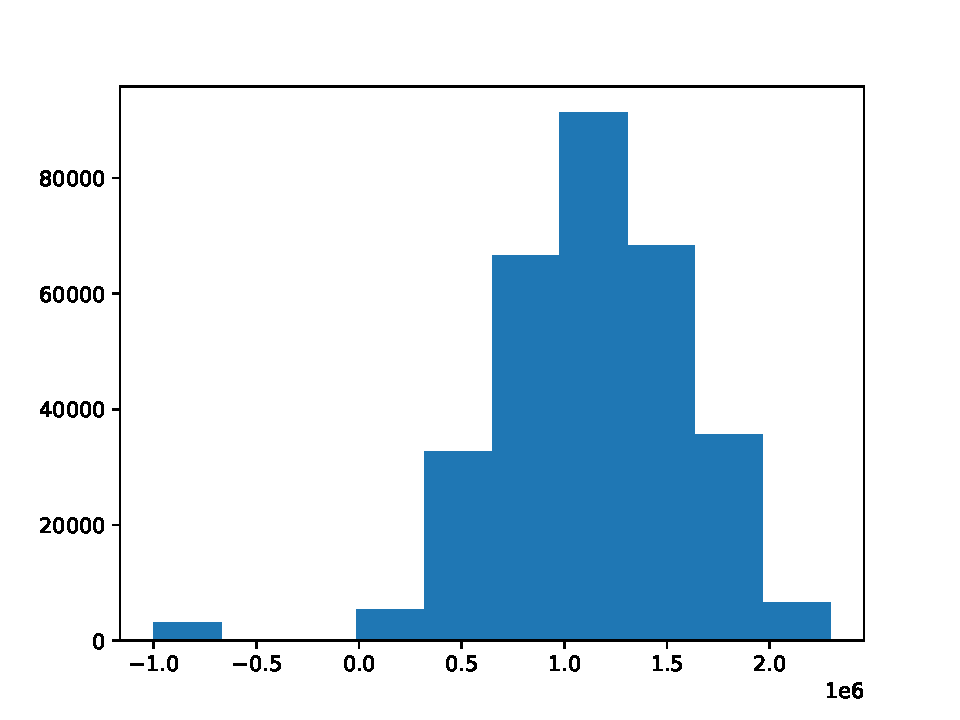
\includegraphics[scale=0.5]{../input/chips_sold}
\par\end{center}

\end{frame}


\section{Conclusion}
\begin{frame}{Conclusion}

\begin{itemize}
\item A
\item B
\item C
\end{itemize}
\end{frame}

\plain{Thank you!}

\end{document}
